\chapter{Data Understanding}
\section*{Der Datensatz}
Gegeben ist der Datensatz ''Daily Financial News for 6000+ Stocks'' mit mehr als einer Millionen Einträgen von englischen Überschriften im Bereich der Aktiennews aus den USA. Die Überschriften sind dabei den jeweiligen Aktien zu geordnet, über welche der Artikel beziehungsweise die Überschrift berichtet.\\ \\
Wir konzentrieren unsere Anstrengungen hinsichtlich der Daten getriebenen Analyse auf den Datensatz ''raw\_analyst\_ratings.csv''.\\
Der Datensatz wird von bot\_developer auf Kaggle.com zur Verfügung gestellt. \\
\citep[siehe][]{dailyfinancialnews}
\begin{figure}
    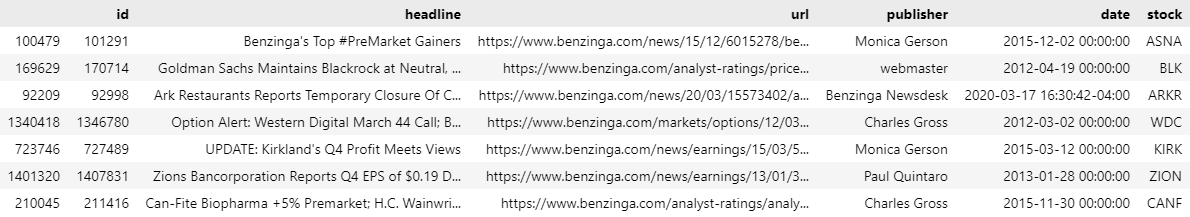
\includegraphics[scale=.49]{img/dataSample7.png}
    \caption{Überblick über den Datensatz, Sieben zufällige Einträge}
\end{figure}
Der oben genannte Datensatz, rawanalystratings, besteht aus sechs Spalten:
\begin{itemize}
    \item \textbf{id}: Eindeutige ID
    \item \textbf{headline}: Überschrift
    \item \textbf{url}: Webseite des Artikels
    \item \textbf{publisher}: Immer Benzinga, daher hier Autor
    \item \textbf{date}: Datum der Veröffentlichung
    \item \textbf{stock}: Die Aktie auf die sich die Überschrift bezieht
\end{itemize}
Eine Überschrift ist immer genau einer Aktie zugeordnet. Die Spalte des Publisher stellt nach Aussage von bot\_developer den Autor da, Publisher ist immer Benzinga \citep[übersetzt][]{dailyfinancialnews}.
Die \textit{id} dient der eindeutigen Identifizierung, da Überschriften und Aktien mehrfach vorkommen und nur die Kombination der beiden features einen eindeutigen Key bilden.
Die \textit{headline} beschreibt den zugrunde liegenden Artikel. Die Artikel selbst sind im Datensatz nicht vorhanden, wie im vorangegangenem Kapitel jedoch erwähnt wollen wir insbesondere die Aussagekraft der Überschrift bewerten. Die Überschrift bezieht sich auf die Veränderung des, ebenfalls im Datensatz genannten \textit{stock}, also der Aktie. Hier ist abzugrenzen, dass die Headlines keine, bzw. nur selten, wirtschaftlichen Geschehnisse des Unternehmens darstellen.
Die \textit{url} und den \textit{publisher} der jeweiligen Headline wird im folgenden nicht weiter betrachtet, verbleibt jedoch im Datensatz zur besseren Nachvollziehbarkeit. Insbesondere zur Abgrenzung der Qualität des Datensatzes, da die fehlende Varietät des Publishers die Allgemeingültigkeit des Modells einschränkt. Die Spalten \textit{date} gibt das Datum der Veröffentlichung der Aktiennews an und ist im folgenden, zusammen mit der Aktienkennung, der Aktie auf die sich die Headline bezieht, essentiell um die Auswirkung der Headline auf eben diese zu evaluieren.\\
Auffällig ist, dass der Datensatz verfügt über keine wertenden Spalten, so ist eine Vorhersage jeglicher Art unmöglich. Es bleibt also im folgenden eine Zielvariable zu bestimmen und für jeden Eintrag zu evaluieren, dies geschieht im Kapitel Data Preparation.

\section*{Überblick}
Insgesamt sind 1407328 Zeilen zu verzeichnen. Diese teilen sich auf 845770 eindeutige Überschriften und 6204 eindeutige Aktien zu 39957 unterschiedlichen Daten auf. Überschriften werden also mehrfach genannt, wenn sich der Artikel auf mehrere Aktien bezieht.\\
Die News stammen aus den Jahren von 2009 bis 2020. Pro Datum fallen etwa 600 bis 1000 Headlines an. Im Schnitt etwa 117277.3 Headlines pro Jahr. Hier zu sehen ist also die fülle von Aktiennews, und dies alleine bei einem Publisher. Ein Wandel der Anzahl über die Jahre ist nur schwer zu erkennen und somit zu vernachlässigen. \\
Die Verteilung der Anzahl der Aktien ist ungleichmäßig so kommen einzelne Aktien wie die ''AADR'', Dorsey Wright ADR ETF, ein ETF der AdvisorShares Investments, LLC, nur zwei Mal vor und andere wie die ''MRK'', die Aktie des Pharmaunternehmens Merck \& Co., bis zu 3238 Mal. \\
\begin{figure}[t]
    \includegraphics[scale=0.25]{img/StockAllocation.png}
    \caption{Boxplot, unaufbereitet}
\end{figure}
Wie in der obenstehenden Grafik zu sehen sind viele Ausreißer der Verteilung zu erkennen, die Durchschnittliche Erwähnung einer Aktie im Zeitraum von 11 Jahren liegt bei unter 200.\\
Die Ungleichverteilung zeigt ein weiteres Spannungsfeld im Bereich des Forschungsthema, wird jedoch im folgenden keinen semantischen Unterschied darstellen, da jede Headline separat in Ihrem Bezug zum jeweiligen Aktienkurs betrachtet wird. Denkbar sind allerdings Zusammenhänge zwischen den Auswirkungen und der Häufigkeit der Veröffentlichung einer Headline zur Aktie. Auch die Betrachtung eines Einflussfaktors der Häufigkeit der Erwähnung einer Aktie in einem kurzen Zeitintervall ist hier zu nennen. \\ \\
Betrachten wir nun die Überschriften ohne diese vorher aufbereitet zu haben, so lassen sich einige Begriffe feststellen, die spezifisch am Aktienmarkt sind, dies muss auf jeden Fall im weiteren Umgang mit den Daten beachtet werden.
So zum Beispiel ''ESP'', was für ''Earnings per share'' steht, also dem Gewinn pro Aktie. Diese Kennzahl wird häufig zur externen Finanzanalyse eines Unternehmens verwendet, hier kann jedoch keine Gewichtung basierend auf dem Wort, bzw. der Abkürzung, getroffen werden. Vor allem auch Begriffe wie ''Price'', ''Stock'', ''Market'' und ''Bezinga'' geben zwar den Kontext der Aktiennews an, da dieser aber ohne hin schon feststeht, wird bei diesen Begriffen keine Gewichtung zum Aktienkurs erwartet. Zumal gängige Sentiment- und Stopword-Dictionarys keine dieser Wörter beinhalten. 
\begin{figure}
    \centering
    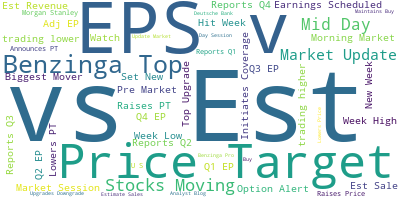
\includegraphics[scale=0.6]{img/wordcloud.png}
    \caption{Top 50 Wörter im gesamten Datensatz, unaufbereitet}
\end{figure}

\section*{Qualität}
Es wurde kein Data Mining betrieben, die Daten stammen aus einer externen Quelle, wie dem obigen Abschnitten zu entnehmen ist.
Die Daten liegen schon in einer bereinigter Form vor und beinhalten keine null-Werte, Duplikate oder Werte die im Kontext keinen Sinn ergeben. Die Zeitstempel allerdings bestehen zum Großteil nur aus tagesgenauen Daten, so sind die Uhrzeiten in 1351341 von 1407328 Fällen (96,02\%) mit ''OO:OO:OO'' angegeben.\\
Mit Hinblick auf die Forschungsfrage, schränkt dieser Tatbestand die Auswahl eines möglichen Vergleichsintervall der potentiellen Zielvariable zur Veröffentlichung der Headline massiv ein. Um einen möglichen Bezug zu der Headline sicher zustellen muss entsprechend der kürzeste Zeitraum um die Veröffentlichung des Artikels gewählt werden.\\
Die Überschriften sind mit reinen ASCII-Zeichen lesbar. \\ 
Laut dem Ersteller des Datensatzes stellt ''Bezinga'' den einzigen Publisher, jedoch sind 1034 verschiedene Publisher zu verzeichnen. Dabei handelt es sich um Autoren bei Bezinga Insights.\\
Während des nächsten Schrittes, der Data Preparation, müssen die Überschriften verarbeitet werden, so dass diese durch maschinenlesbare Attribute abgebildet werden. Hier muss darauf geachtet werden, dass die gängigen Verfahren der Sentiment- oder Stopword-Dictionarys die aktienmarkt-spezifischen Wörter nicht vollständig abdecken werden. Insbesondere die Wechselwirkungen auf dem Aktienmarkt werden durch Wörter abgebildet, die durch das Verfahren des Stopword-Removal entfernt werden \citep{sentimentTagTowards}. Darüber hinaus ist eine Evaluation des Zeitraumes zwischen einer möglichen Zielvariable und der Veröffentlichung der Aktiennews nur tageweise möglich.